% !TeX program = xelatex
\documentclass[11pt,a4paper]{article}
\usepackage[a4paper,left=25mm,right=25mm,top=22mm,bottom=22mm]{geometry}
\usepackage{fontspec}
\IfFontExistsTF{Latin Modern Roman}{\setmainfont{Latin Modern Roman}}{\setmainfont{Times New Roman}}
\IfFontExistsTF{Latin Modern Mono}{\setmonofont{Latin Modern Mono}[Scale=MatchLowercase]}{\setmonofont{Consolas}[Scale=MatchLowercase]}
\usepackage{graphicx,booktabs,longtable,array}
\usepackage[hidelinks]{hyperref}
\hypersetup{pdftitle={Task 1: Anti-Cheat Detection},pdfauthor={Team ML003}}
\setlength{\parindent}{1.35em}
\setlength{\parskip}{2pt}
\setlength{\tabcolsep}{6pt}
\renewcommand{\arraystretch}{1.22}
\setlength{\emergencystretch}{2em}
\setlength{\abovecaptionskip}{5pt}
\setlength{\belowcaptionskip}{2pt}
\makeatletter
\let\@afterindentfalse\@afterindenttrue
\newcommand{\inlinefigurecaption}[1]{%
  \begingroup
  \def\@captype{figure}%
  \long\def\@makecaption##1##2{%
    \vskip\abovecaptionskip
    {\centering ##1: ##2\par}%
    \vskip\belowcaptionskip
  }%
  \caption{#1}%
  \endgroup
}
\makeatother
\newcolumntype{L}[1]{>{\raggedright\arraybackslash}p{#1}}
\newcommand{\reserveheading}[1]{\par\ifdim\dimexpr\pagegoal-\pagetotal\relax<#1\relax\newpage\fi}
\setcounter{secnumdepth}{3}
\begin{document}
\raggedbottom
\begin{center}
CPE342 Machine Learning\par
\vspace{5pt}
{\Large\bfseries Task 1: Anti-Cheat Detection\par}
\vspace{5pt}
{\normalsize\bfseries Team ML003\par}
\end{center}
\vspace{6pt}

\section{Problem and Dataset}

Task 1 uses gameplay and account features to identify cheaters. The target variable, \texttt{is\_\allowbreak{}cheater}, is \texttt{0} for legitimate players and \texttt{1} for cheaters. This is a binary classification problem. The primary metric is \textbf{binary F2}, which gives more weight to recall because missing cheaters is a concern.

The training set contains 104,000 rows, including 90,816 labeled rows and 13,184 unlabeled rows (12.7\%). Among the labeled rows, 34.9\% are cheaters and 65.1\% are legitimate players. The test set contains 25,889 rows. The 31 raw features include gameplay statistics such as \texttt{kill\_\allowbreak{}death\_\allowbreak{}ratio} and \texttt{reaction\_\allowbreak{}time\_\allowbreak{}ms}, and account characteristics such as \texttt{reports\_\allowbreak{}received} and \texttt{account\_\allowbreak{}age\_\allowbreak{}days}.

\section{Methodology}

\subsection{Exploratory Data Analysis}

We first checked which rows had labels and how the classes were distributed. We then examined which predictors distinguish the classes and how much information remains when values are missing.

\reserveheading{6\baselineskip}
\subsubsection*{1. Class Balance}

We counted the labeled and unlabeled rows, then compared the two classes within the labeled subset.

\par\medskip\noindent\begin{minipage}{\linewidth}
\centering
\hypertarget{task1-figure-1}{}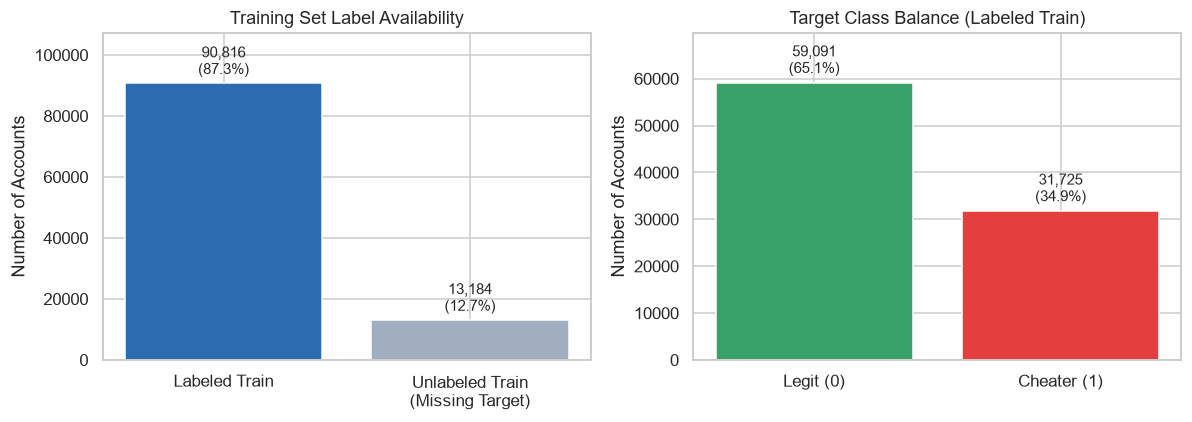
\includegraphics[width=\linewidth,height=0.35\textheight,keepaspectratio]{task1_figures/class_balance.png}
\inlinefigurecaption{Label availability (left) and class balance among labeled rows (right)}
\end{minipage}\par\medskip

In \hyperlink{task1-figure-1}{Figure 1}, the left panel shows 13,184 unlabeled training rows (12.7\%). The right panel shows that 34.9\% of the labeled rows are cheaters. We use the labeled rows for supervised training and stratify the folds to preserve that class proportion. Model A also uses unlabeled rows to estimate the distributions of account age and level.

\reserveheading{0.41\textheight}
\subsubsection*{2. Feature Signal}

We evaluated all 31 raw features individually using ROC-AUC. Taking the greater of AUC and 1 \ensuremath{-} AUC captures separation in either direction.

\par\medskip\noindent\begin{minipage}{\linewidth}
\centering
\hypertarget{task1-figure-2}{}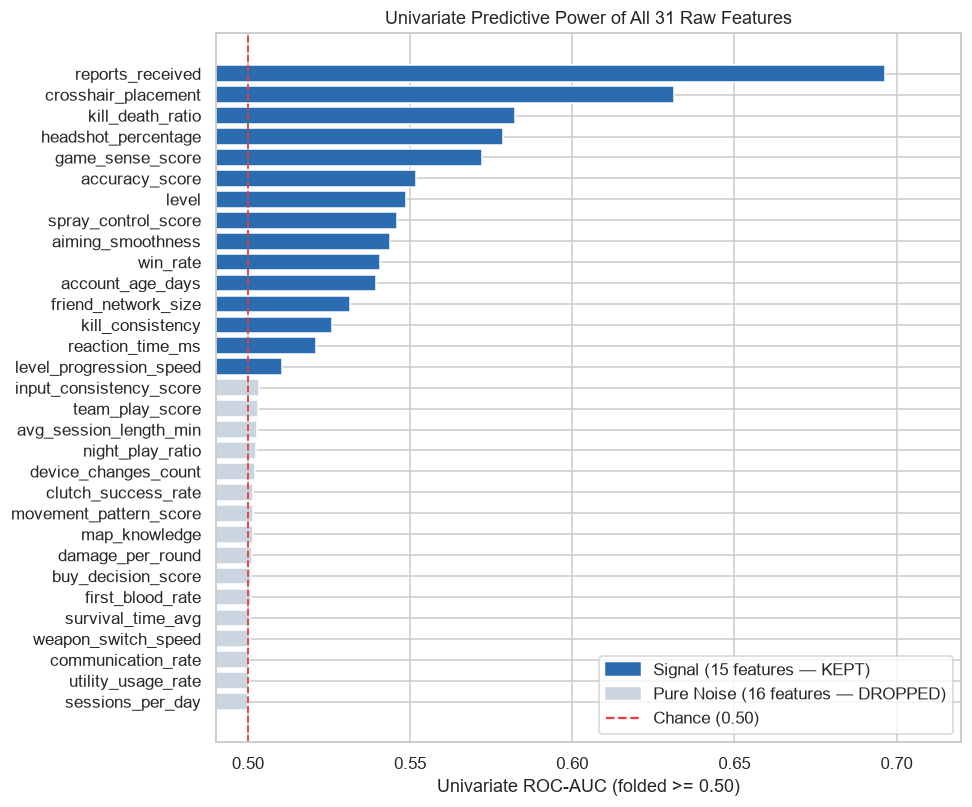
\includegraphics[width=\linewidth,height=0.35\textheight,keepaspectratio]{task1_figures/feature_signal.png}
\inlinefigurecaption{Folded univariate ROC-AUC for the 15 retained and 16 excluded predictors}
\end{minipage}\par\medskip

In \hyperlink{task1-figure-2}{Figure 2}, \texttt{reports\_\allowbreak{}received} and \texttt{crosshair\_\allowbreak{}placement} have the highest folded ROC-AUC. The 15 retained predictors range from 0.5106 to 0.6965, while the other 16 cluster near 0.5. This screening step reduces the raw feature set from 31 to 15 before feature engineering.

\reserveheading{6\baselineskip}
\subsubsection*{3. Missingness}

We compared feature missing rates and measured the cheater rate among rows with and without an observed value.

\par\medskip\noindent\begin{minipage}{\linewidth}
\centering
\hypertarget{task1-figure-3}{}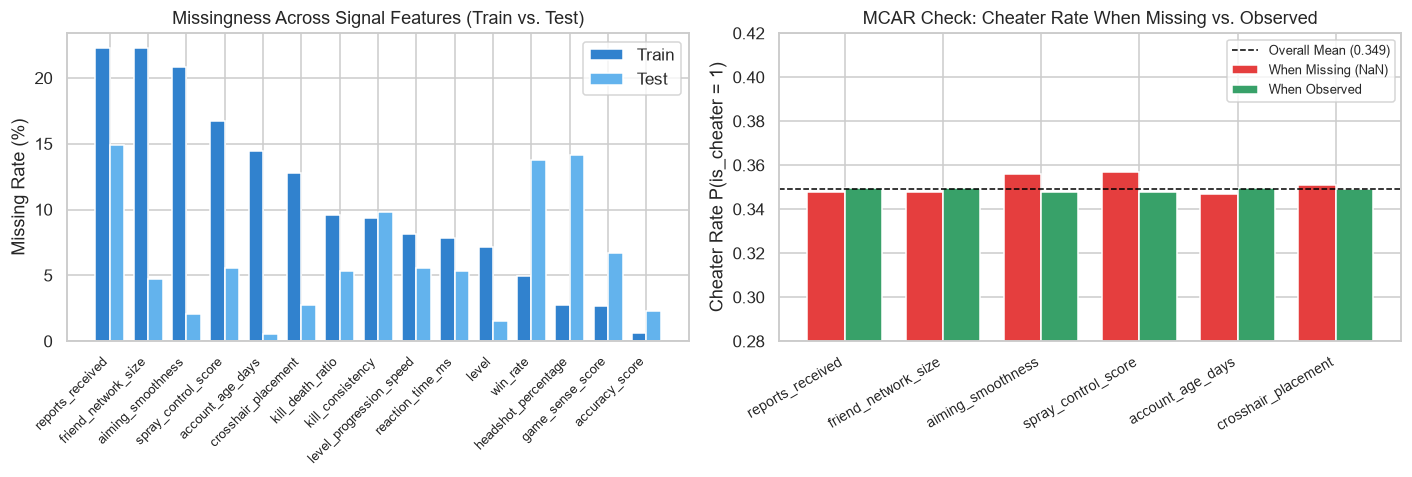
\includegraphics[width=\linewidth,height=0.35\textheight,keepaspectratio]{task1_figures/missingness.png}
\inlinefigurecaption{Missing rates in train and test (left) and cheater rates with and without observed values (right)}
\end{minipage}\par\medskip

In the left panel of \hyperlink{task1-figure-3}{Figure 3}, \texttt{reports\_\allowbreak{}received} and \texttt{friend\_\allowbreak{}network\_\allowbreak{}size} are each missing in about 22\% of labeled training rows. Both have lower missing rates in test. In the right panel, the cheater rate for \texttt{reports\_\allowbreak{}received} is close to 35\% whether the value is missing or observed. This comparison alone cannot establish that values are missing completely at random (MCAR). Model A uses missing indicators and masks additional values during training so it can learn from incomplete records.

\reserveheading{0.41\textheight}
\subsubsection*{4. Class-Exclusive Ranges}

We compared the distributions of \texttt{reports\_\allowbreak{}received}, \texttt{crosshair\_\allowbreak{}placement}, \texttt{level}, and \texttt{account\_\allowbreak{}age\_\allowbreak{}days} by class.

\par\medskip\noindent\begin{minipage}{\linewidth}
\centering
\hypertarget{task1-figure-4}{}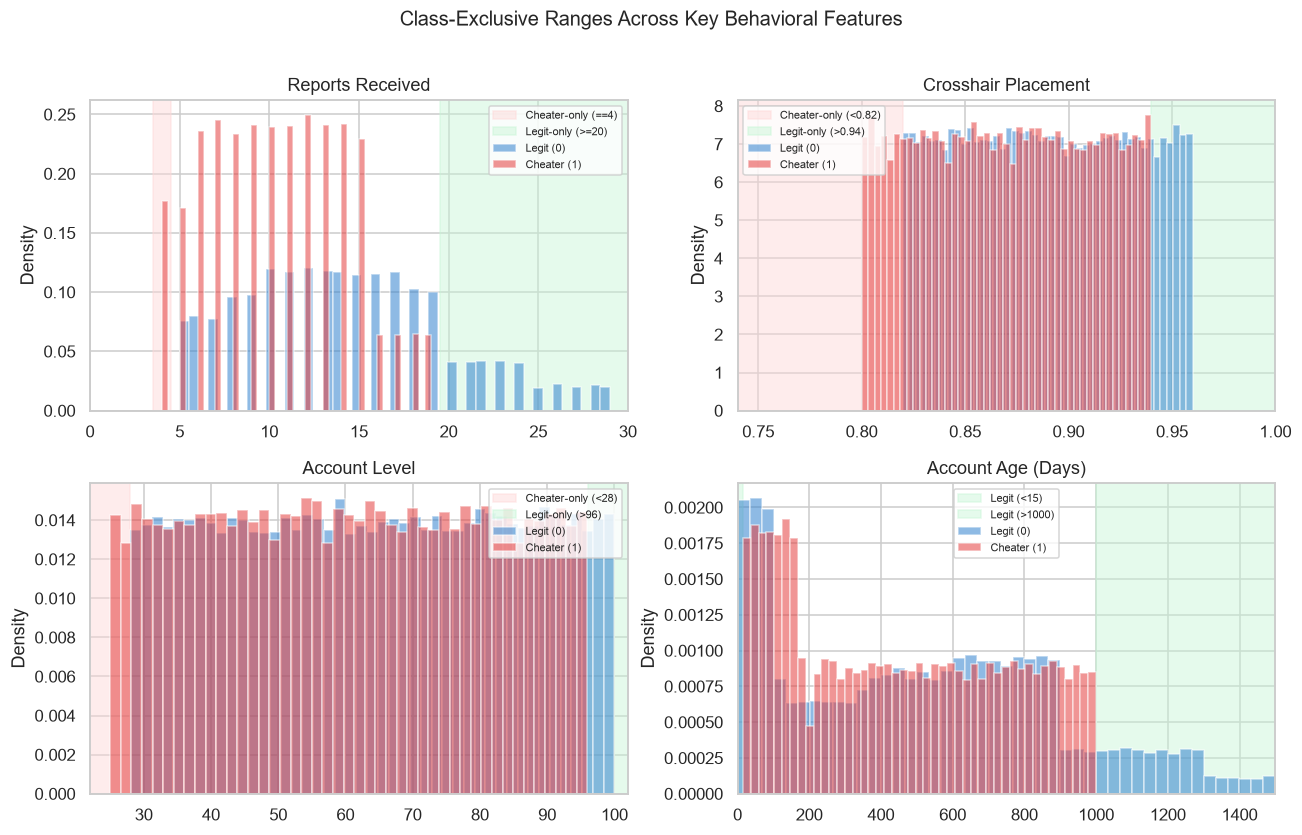
\includegraphics[width=.89\linewidth,height=0.35\textheight,keepaspectratio]{task1_figures/behavioral_ranges.png}
\inlinefigurecaption{Feature distributions by class, with class-exclusive ranges shaded}
\end{minipage}\par\medskip

The shaded bands in \hyperlink{task1-figure-4}{Figure 4} mark ranges where only one class was observed in the training data. For example, \texttt{reports\_\allowbreak{}received == 4} and \texttt{level < 28} occur among cheaters, while \texttt{reports\_\allowbreak{}received >= 20} and \texttt{level > 96} occur among legitimate players. The distributions overlap in other ranges. The pipeline captures these patterns with \texttt{zone\_\allowbreak{}cheat} and \texttt{zone\_\allowbreak{}legit} and groups account ages with \texttt{age\_\allowbreak{}segment}.

\reserveheading{6\baselineskip}
\subsubsection*{5. Algebraic Relationship}

For rows with all three values present, we computed \texttt{r = level\_\allowbreak{}progression\_\allowbreak{}speed \ensuremath{\times} account\_\allowbreak{}age\_\allowbreak{}days / level} to see whether two observed values could constrain a third missing value.

\par\medskip\noindent\begin{minipage}{\linewidth}
\centering
\hypertarget{task1-figure-5}{}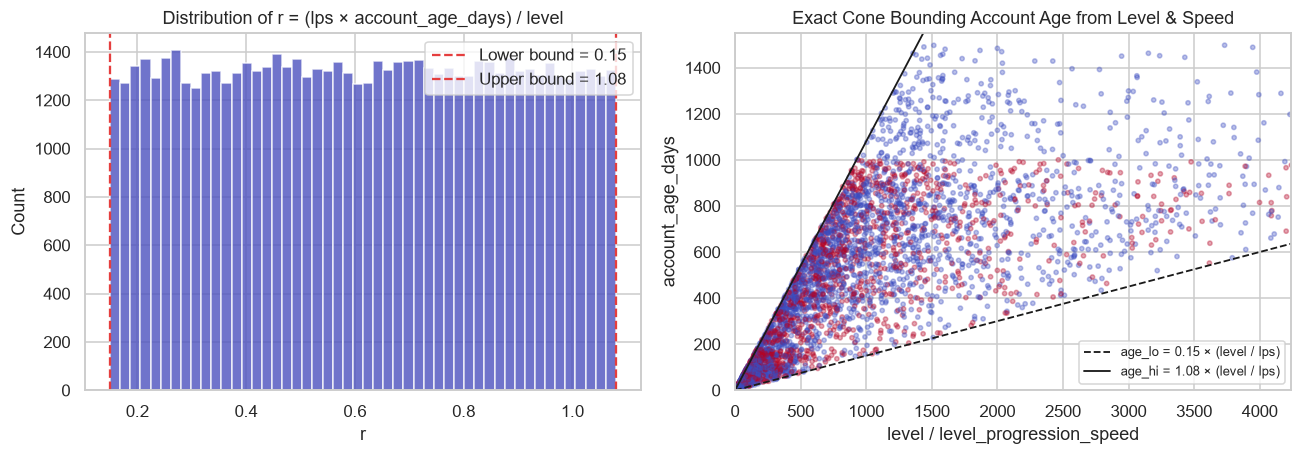
\includegraphics[width=.89\linewidth,height=0.35\textheight,keepaspectratio]{task1_figures/age_bounds.png}
\inlinefigurecaption{Distribution of r (left) and bounds for observed account age (right)}
\end{minipage}\par\medskip

The left panel of \hyperlink{task1-figure-5}{Figure 5} shows \texttt{r} spread nearly evenly between 0.15 and 1.08. In the right panel, those limits define two lines that bound the observed account age at a given ratio of \texttt{level} to \texttt{level\_\allowbreak{}progression\_\allowbreak{}speed}. If age is missing, the same limits give a feasible age range. Rearranging the equation gives bounds for a missing level. Model A uses these bounds to estimate missing values and calculate the probability of falling in each zone.

\reserveheading{10\baselineskip}
\subsection{Preprocessing and Feature Engineering}

The EDA findings lead to five decisions in the training pipeline.
\par\medskip\noindent
\begin{tabular}{@{}L{.35\linewidth}L{.59\linewidth}@{}}
\toprule
\textbf{EDA evidence} & \textbf{Pipeline decision} \\
\midrule
\hyperlink{task1-figure-1}{Figure 1}. Class balance & Train on labeled rows and preserve class proportions in each fold. \\
\hyperlink{task1-figure-2}{Figure 2}. Feature signal & Keep 15 of the 31 raw predictors. \\
\hyperlink{task1-figure-3}{Figure 3}. Missingness & Add missing indicators and train Model A on additional masked rows. \\
\hyperlink{task1-figure-4}{Figure 4}. Class-exclusive ranges & Encode the observed ranges with zone flags and age bins. \\
\hyperlink{task1-figure-5}{Figure 5}. Bounds on age and level & Use the two observed values to constrain the missing third value. \\
\bottomrule
\end{tabular}\par\medskip

\subsubsection*{1. Training rows and raw predictors}

We excluded \texttt{player\_\allowbreak{}id} and \texttt{is\_\allowbreak{}cheater} from the predictors and retained the 15 raw features identified in \hyperlink{task1-figure-2}{Figure 2}. Before splitting the data into folds, Model A computed medians, standard deviations, frequency tables, and marginal priors from the full training set, including unlabeled rows. Model C used the labeled training set to compute its statistics and quantile bin edges, and aligned category levels between the training and test sets before fitting.

\subsubsection*{2. Missing values}

Models A and C retained \texttt{NaN} in the raw predictors for the tree models to handle. We added \texttt{na\_\allowbreak{}*} indicators for \texttt{reports\_\allowbreak{}received}, \texttt{friend\_\allowbreak{}network\_\allowbreak{}size}, \texttt{account\_\allowbreak{}age\_\allowbreak{}days}, \texttt{crosshair\_\allowbreak{}placement}, and \texttt{level}. The feature \texttt{n\_\allowbreak{}missing} counts missing values across the 15 retained raw features.

\subsubsection*{3. Bounds for missing values}

Let \texttt{lps = level\_\allowbreak{}progression\_\allowbreak{}speed}. The limits shown in \hyperlink{task1-figure-5}{Figure 5} give the age bounds \texttt{[level \ensuremath{\times} 0.15 / lps, level \ensuremath{\times} 1.08 / lps]} and the level bounds \texttt{[lps \ensuremath{\times} age / 1.08, lps \ensuremath{\times} age / 0.15]}. The derived features \texttt{age\_\allowbreak{}filled} and \texttt{lvl\_\allowbreak{}filled} use the geometric mean of the corresponding bounds when the original value is missing and retain the observed value otherwise.

\subsubsection*{4. Zone indicators and Bayesian zone posteriors}

The indicators \texttt{zone\_\allowbreak{}cheat} and \texttt{zone\_\allowbreak{}legit} use ranges identified in \hyperlink{task1-figure-4}{Figure 4}, while \texttt{age\_\allowbreak{}segment} bins accounts by age. When age or level is missing and the other two inputs are present, Model A evaluates candidate ages in one-day increments or candidate levels in increments of 0.1. It excludes candidates that violate the limits on \texttt{r} in \hyperlink{task1-figure-5}{Figure 5}. For the remaining candidates, the implementation multiplies the empirical prior by the candidate age or divides it by the candidate level, then normalizes the weights to sum to one.

The total weight in an interval such as \texttt{110 <= account\_\allowbreak{}age\_\allowbreak{}days < 120} produces a \texttt{pa\_\allowbreak{}*} or \texttt{pl\_\allowbreak{}*} feature. The weighted means become \texttt{age\_\allowbreak{}post\_\allowbreak{}mean} and \texttt{lvl\_\allowbreak{}post\_\allowbreak{}mean}. For observed values, the zone probabilities are 0 or 1 according to the interval containing the value.

\reserveheading{11\baselineskip}
\subsubsection*{5. Additional features}

Models A and C use the transformations in Table 1. Model A has 56 features after the posterior features are included.

\begingroup\small
\begin{longtable}{@{}L{.22\linewidth}L{.73\linewidth}@{}}
\toprule
\textbf{Transformation} & \textbf{Examples and Rationale} \\
\midrule
\endfirsthead
\toprule
\textbf{Transformation} & \textbf{Examples and Rationale} \\
\midrule
\endhead
\bottomrule
\endfoot
Rates per 100 Days & \texttt{reports\_\allowbreak{}per\_\allowbreak{}100d}, \texttt{friends\_\allowbreak{}per\_\allowbreak{}100d}, and \texttt{level\_\allowbreak{}per\_\allowbreak{}100d} use account age plus one in the denominator so the rates can be compared across accounts of different ages. \\
Interactions & \texttt{kd\_\allowbreak{}x\_\allowbreak{}hs} multiplies \texttt{kill\_\allowbreak{}death\_\allowbreak{}ratio} by \texttt{headshot\_\allowbreak{}percentage}. \texttt{acc\_\allowbreak{}x\_\allowbreak{}cross} multiplies \texttt{accuracy\_\allowbreak{}score} by \texttt{crosshair\_\allowbreak{}placement}. \\
Skill Summary & \texttt{skill\_\allowbreak{}z\_\allowbreak{}sum} sums available skill values after scaling them with training medians and standard deviations, provided at least three values are present. \texttt{skill\_\allowbreak{}z\_\allowbreak{}std} summarizes their spread. \\
Frequencies and Log Transform & \texttt{freq\_\allowbreak{}reports} and \texttt{freq\_\allowbreak{}friends} encode frequencies from the training data. Separate \texttt{log1p} features transform account age, friend count, progression speed, and report count. \\
\end{longtable}
\endgroup

{\centering\small Table 1. Engineered feature groups and their purpose\par}\medskip

\subsubsection*{6. Masking augmentation}

To expose Model A to incomplete records like those in \hyperlink{task1-figure-3}{Figure 3}, each fold uses four copies of the fitting rows and randomly masks values at the per-feature missing rates measured in the labeled training set. The pipeline rebuilds the engineered features with \texttt{build\_\allowbreak{}features\_\allowbreak{}full} and retains the original labels. Masking is limited to these copies so that early stopping, outer validation, and test prediction use the original observations.

\reserveheading{11\baselineskip}
\subsection{Model Design and Validation}

The ensemble gives 70\% of the weight to the masked LightGBM and uses the other two components to combine alternative representations of the data. Table 2 gives the weights and the composition of each component.

\begingroup\small
\begin{longtable}{@{}L{.15\linewidth}L{.11\linewidth}L{.67\linewidth}@{}}
\toprule
\textbf{Component} & \textbf{Weight} & \textbf{Training and Preprocessing} \\
\midrule
\endfirsthead
\toprule
\textbf{Component} & \textbf{Weight} & \textbf{Training and Preprocessing} \\
\midrule
\endhead
\bottomrule
\endfoot
Model A & 0.70 & LightGBM with masking augmentation and multi-seed bagging. \\
Model B & 0.20 & Logistic regression stack over LightGBM, ExtraTrees, a PyTorch MLP, and a spline-based linear SVM. \\
Model C & 0.10 & Blend of tuned XGBoost, LightGBM, and CatBoost with categorical features. \\
\end{longtable}
\endgroup

{\centering\small Table 2. Model components and their weights in the final ensemble\par}\medskip

\textbf{Model A.} Stratified five-fold cross-validation uses seeds 42, 7, and 2024. Each fold is fitted three times at a learning rate of 0.02. Each fit reserves 10\% of its training portion for early stopping on ROC-AUC. The test scores average 45 fitted models.

\textbf{Model B.} ExtraTrees fills missing values with \texttt{-1}. The MLP uses median imputation and quantile transformation, while the SVM uses median imputation, standardization, and spline features. Each base model generates out-of-fold (OOF) scores on rows held out from its fit. A logistic regression stack is trained in five folds on the four base models' OOF logits. For test prediction, the meta-model is fitted on all base OOF logits.

\textbf{Model C.} XGBoost, LightGBM, and CatBoost use five folds and blend weights of 0.1834, 0.4848, and 0.3318, respectively. The feature set includes \texttt{reports\_\allowbreak{}cat} and \texttt{age\_\allowbreak{}segment}, with quantile bins for \texttt{friends\_\allowbreak{}bin}, \texttt{level\_\allowbreak{}bin}, and \texttt{crosshair\_\allowbreak{}bin}.

\reserveheading{7\baselineskip}
\subsection{Evaluation Metrics and Threshold Selection}

ROC-AUC evaluates ranking before a threshold is chosen. Binary F2 evaluates the resulting classifications with \texttt{is\_\allowbreak{}cheater = 1} as the positive class. In \texttt{5TP / (5TP + 4FN + FP)}, TP denotes a cheater correctly flagged, FN denotes a cheater missed, and FP denotes a legitimate account flagged. The larger weight on FN reflects the emphasis on recall.

The component scores have different distributions. Before blending, we use each model's out-of-fold (OOF) empirical cumulative distribution function (ECDF) to express its scores as percentiles on a common scale. For Model C, this transformation is applied to each base model and then to the combined score. Models A, B, and C are blended with weights \textbf{0.70 / 0.20 / 0.10}. The resulting \texttt{score} ranks accounts on a common scale. A score of 0.70 does not establish a 70\% probability of cheating.

We evaluated 251 candidate thresholds across quantiles 0.20–0.70 of the blended OOF scores. The threshold that maximized binary F2 was \textbf{0.37264}. We applied it to the test scores and saved \texttt{id}, \texttt{pred}, and \texttt{score} in \texttt{task1\_\allowbreak{}predictions.csv}.

\reserveheading{16\baselineskip}
\subsection{Results}

\begingroup\small
\begin{longtable}{@{}L{.47\linewidth}L{.20\linewidth}L{.24\linewidth}@{}}
\toprule
\textbf{Model} & \textbf{OOF ROC-AUC} & \textbf{OOF Binary F2} \\
\midrule
\endfirsthead
\toprule
\textbf{Model} & \textbf{OOF ROC-AUC} & \textbf{OOF Binary F2} \\
\midrule
\endhead
\bottomrule
\endfoot
Model A · LightGBM with Masking & 0.89482 & — \\
Model B · Logistic Regression Stack & 0.89283 & — \\
Model C - XGBoost base learner & 0.89128 & — \\
Model C - LightGBM base learner & 0.89193 & — \\
Model C - CatBoost base learner & 0.89116 & — \\
Final A/B/C Ensemble & \textbf{0.89501} & \textbf{0.83979} \\
\end{longtable}
\endgroup

{\centering\small Table 3. OOF results for recorded model components and the final ensemble\par}\medskip

\textbf{Ranking.} Table 3 shows an OOF ROC-AUC gain of \textbf{0.00019} over Model A.

\textbf{Classification.} The ensemble reached \textbf{0.83979} binary F2 at an OOF threshold of \textbf{0.37264}. The component F2 values were not reported, so Table 3 cannot establish an F2 gain over Model A.

\textbf{Review volume.} The same threshold flagged \textbf{62.80\%} of OOF accounts and \textbf{59.81\%} of test accounts. These are the shares sent for review if every flagged account is investigated.

\subsection{Pipeline Improvement}

\subsubsection*{1. Base Learner Comparison}

The A/B/C labels group multiple learners rather than three single algorithms. Model B stacks LightGBM (OOF ROC-AUC 0.89285), ExtraTrees (0.86112), PyTorch MLP (0.84681), and spline LinearSVC (0.83907) with logistic regression; the stack reached 0.89283. Model C's XGBoost, LightGBM, and CatBoost base-learner scores are listed in Table 3. Each recorded Model C learner and the Model B stack scored below Model A.

\subsubsection*{2. Input and Score Processing}

Preprocessing differed by learner: Model A uses four randomly masked copies per fitting fold; Model B uses learner-specific imputation and transformations; Model C adds categorical quantile bins. The feature-engineering methods are described in Section 2.2. After prediction, ECDF alignment puts component scores on a common scale before the weighted blend; the OOF F2 threshold selection is described in Section 2.4.

\subsubsection*{3. What the Comparison Shows}

The final blend improves OOF ROC-AUC by 0.00019 over Model A (Table 3). Component F2 values, a raw-feature baseline, and isolated ablations were not recorded, so the comparison cannot identify which learner or preprocessing step produced the gain or establish a component-level F2 improvement.

\subsection{Error Analysis and Limitations}

The overlap in \hyperlink{task1-figure-4}{Figure 4} identifies feature ranges worth examining for classification errors. The reported results are aggregate scores. To determine where errors are concentrated, we would need to count false positives and false negatives by feature range and missingness pattern.

The reported binary F2 reflects threshold selection and evaluation on the same OOF scores. In addition, Model A's reference statistics and Model C's quantile bin edges were computed before the folds were split, while Model B trained its meta-model on a precomputed set of base OOF scores. A separate holdout would let us evaluate the selected threshold on rows that played no part in choosing it. Alternatively, preprocessing, stacking, and threshold selection could all be fitted within nested cross-validation.

\reserveheading{13\baselineskip}
\section{Insights and Common Mistakes}

\begin{itemize}
\item \textbf{Interpret univariate AUC at the feature level.} The values near 0.5 in \hyperlink{task1-figure-2}{Figure 2} indicate weak ranking performance for a feature on its own. Model comparisons are needed to assess whether it adds information in combination with other features.
\item \textbf{Distinguish masking from estimation.} \hyperlink{task1-figure-3}{Figure 3} motivated random masking during training. \hyperlink{task1-figure-5}{Figure 5} provides bounds for estimating a missing age or level when the other two values are known.
\item \textbf{Compare gains with the cost of additional models.} Table 3 shows a small ROC-AUC gain over Model A. A separate comparison of binary F2 and runtime would help determine whether the three-component ensemble is worthwhile.
\end{itemize}

\section{Domain Interpretation and Business Impact}

An anti-cheat team could use \texttt{score} to prioritize account reviews and \texttt{pred} to identify accounts at or above the competition threshold. The 59.81\% test flag rate reported in Results means that the competition threshold would send nearly six out of ten accounts into the review queue. An operational threshold should reflect review capacity and the cost of missing a cheater. The class-exclusive ranges in \hyperlink{task1-figure-4}{Figure 4} should also be checked on live player data before they inform account decisions.

\section{Conclusion}

The relationship in \hyperlink{task1-figure-5}{Figure 5} lets the model use two observed account features to constrain a third when it is missing. Masking complements that step by exposing LightGBM to incomplete records during training. The final ensemble adds \textbf{0.00019} OOF ROC-AUC over Model A. Table 3 leaves open whether that gain carries over to the competition metric, binary F2.

To decide whether to keep the ensemble, compare it with Model A on a separate holdout using binary F2, runtime, and the share of accounts flagged. Break down precision and recall by missingness pattern and by the overlapping ranges in \hyperlink{task1-figure-4}{Figure 4} to show where either model needs improvement.
\end{document}
